\documentclass[10pt,twocolumn]{article} 
\usepackage{simpleConference}
\usepackage{fancyhdr}
\usepackage{amsmath,amsfonts,amssymb,graphicx}
\usepackage{subfigure}   % 使用子图形
\usepackage{indentfirst} % 中文段落首行缩进
\usepackage{bm}          % 公式中的粗体字符(用命令\boldsymbol）
\usepackage{indentfirst} % 中文首段缩进
\usepackage{abstract}    % 2栏文档，一栏摘要及关键字宏包
\usepackage{amsthm}      % 使用定理
\usepackage{booktabs}    % 使用表格
\usepackage{siunitx}
\usepackage{tikz}
\usepackage{enumitem}
\usepackage{titlesec}
\usepackage{times}
\usepackage{wasysym}
\usepackage{pifont}
\usepackage{ccaption}
\usepackage{float}
\usepackage{calc}
\usetikzlibrary{calc}
\usetikzlibrary{circuits.ee.IEC}
% 在导言区添加 circuitikz 包
\usepackage{circuitikz}
\usepackage{environ}
\usepackage{lmodern}
\usepackage{anyfontsize}
\usepackage{hyperref}
\usepackage{tabu}
\usepackage{tabularx}
\usepackage{multirow}
\usepackage{multicol}
\usepackage{longtable}
\usepackage{makecell}
\usepackage{graphicx}
\usepackage{amssymb}
\usepackage{ragged2e}
\usepackage{url,hyperref}

\newcommand*{\effXsecDPS}{\sigma_{\text{eff,DPS}}}
\newcommand*{\effXsecTPS}{\sigma_{\text{eff,TPS}}}
\newcommand*{\effXsecNPS}{\sigma_{\text{eff,NPS}}}
\newcommand*{\GeV}{~\text{GeV}}
\newcommand*{\GeVc}{~\text{GeV/c}}
\newcommand*{\GeVcs}{~\text{GeV}\text{c}^2}
\newcommand*{\TeV}{~\text{TeV}}
% \newcommand*{\d}{\mathrm{d}}
\newcommand*{\mb}{~\text{mb}}
\newcommand*{\fb}{~\text{fb}}
\newcommand*{\ifb}{~\text{fb}^{-1}}

\renewcommand{\arraystretch}{1.2}

\begin{document}

\title{Double, Triple, and $n$-Parton Scattering Processes in High-Energy Proton-Proton Collisions}

\author{Chi Wang
\\
Zhili College, Tsinghua University
\\
2022012259, chi-wang22@mails.tsinghua.edu.cn
\\
\\
14th January, 2026
\\
}

\maketitle
\thispagestyle{empty}

\begin{abstract}

$n$-Parton Scattering (NPS) processes in high-energy proton-proton collisions serve as a vital tool for probing the complex internal structure of the proton. This report reviews the current theoretical frameworks and experimental status of NPS, with a primary focus on double parton scattering (DPS) and triple parton scattering (TPS). We discuss the standard "pocket formula" formalism and the effective cross-section $\sigma_{\text{eff}}$, highlighting the significant discrepancies observed in $\sigma_{\text{eff,DPS}}$ measurements between jet-based and quarkonium-based processes. The theoretical relationships between DPS and TPS effective cross-sections are examined, along with recent experimental milestones such as the observation of triple-$J/\psi$ production. Finally, we explore the potential of using data from LHC Run 3 to perform measurements in novel channels to enhance our understanding of parton dynamics inside protons.

\end{abstract}


\section{Introduction}

Proton consists of three quarks, two up-type and one down-type, and gluons, which hold together the three valence quarks, as well as of a 'sea' of virtual quark-antiquark pairs.
These components are referred to as 'partons' and can be probed in proton-proton hard scatterings.
In the standard picture of proton-proton collisions, typically only one pair of partons undergo a hard scattering with each another, with the remainders of each proton only slightly disturbed in the process.
As the collision energy increases, the densities of gluons and sea quarks probed inside each proton grow rapidly. Thus, at higher collision energies, it becomes more likely for more than one pair of partons undergo a hard scattering in a single pp collision, leading to the simultaneous and independent production of two or more particles with transverse momentum ($p_T$) and/or mass ($m$) above a few giga-electronvolts.
Such processes are collectively referred to as $n$-parton scattering (NPS).

NPS processes offer an important probe into the complicated inner structure of the proton and its evolution with energy.\cite{DIEHL_MPI}\cite{BLOK_MPS} Many of these features, for example, the parton density profile in the plane transverse to the colliding beams, as well as the various correlations (in position, momentum, flavour, colour, spin and so on) between individual partons, are very difficult to calculate theoretically, since QCD behaves non-perturbatively in low-energy regions, and can only be mapped out through experimental studies of NPS in different systems and for different numbers $n$ of simultaneous scatterings \cite{MPI_LHC}.

In addition to providing an insight into proton structure, NPS studies also contributes to background subtraction in future searches for rare standard model and beyond-standard model resonances, especially at future hadron colliders, where the NPS contribution to the backgound becomes more significant due to higher centre-of-mass energy.\cite{DdE_TPS}\cite{YJZ_TRI_JPSI}

\section{\texorpdfstring{Theoretical Framework of $n$-Parton Scattering}{Theoretical Framework of n-Parton Scattering}}

In a generic hadronic collision, the inclusive cross section for $n$ independent hard parton scatterings can be written as a convolution of generalized $n$-parton distribution functions (PDF) and elementary partonic cross sections summed over all involved partons:
\begin{equation}
    \label{eqn:nps_general}
    \begin{aligned}
        &
            \sigma_{hh'\to a_1\dots a_n}^{\text{NPS}} 
        \\
        =
        &
            \left(\frac{m}{n!}\right) \sum_{i_1,\dots,i_n,i'_1,\dots,i'_n} \int \mathrm{d} x_1 \cdots \mathrm{d} x_n \mathrm{d} x'_1 \cdots \mathrm{d} x'_n
        \\
        &
            \times \mathrm{d}^2 \mathbf{b_1} \cdots \mathrm{d}^2 \mathbf{b_n} \mathrm{d}^2 \mathbf{b}
        \\
        &
            \times \Gamma_h^{i_1\dots i_n}(x_1,\dots,x_n;\mathbf{b_1},\dots,\mathbf{b_n};Q_1^2,\dots,Q_n^2)
         \\
        &
            \times \hat{\sigma_{a_1}^{i_1 i'_1}(x_1,x'_1,Q_1^2)}\cdots \hat{\sigma}_{a_n}^{i_n i'_n}(x_n,x'_n,Q_n^2)
        \\
        &
            \times \Gamma_{h'}^{i'_1\dots i'_n}(x'_1,\dots,x'_n;\mathbf{b_1}-\mathbf{b},\dots,\mathbf{b_n}-\mathbf{b};Q_1^2,\dots,Q_n^2)
    \end{aligned}
\end{equation}

Here, $\Gamma_h^{i_1\dots i_n}(x_1,\dots,x_n;\mathbf{b_1},\dots,\mathbf{b_n};Q_1^2,\dots,Q_n^2)$ are $n$-parton generalized distribution functions, dependent on the momentum fractions $x_1, \dots, x_n$, and energy scales $Q_1,\dots,Q_n$, at transverse positions $\mathbf{b_1}, \dots, \mathbf{b_n}$ of the partons, producing final-state particles $a_1, \dots, a_n$ with each subprocess cross section being $\hat{\sigma}_{a_1}^{i_1i'_1}, \dots, \hat{\sigma}_{a_n}^{i_ni'_n}$, respectively.
The combinatorial factor $\mathfrak{m}/n!$ accounts for the indistinguishability of the final-state particles, when identical particles are produced.

The $n$-parton distribution function $\Gamma_h^{i_1\dots i_n}$ encodes, in principle, all the 3D parton structure of the hadron of relevance to compute the NPS cross-sections, describing the parton densities in the transverse plane and/or any parton correlations in kinematical and/or quantum-number spaces.
Yet, the non-perturbative behaviour of QCD and the many-body nature of the system complicate the direct derivation of the function, and subsequently the NPS cross-sections.

A common approach is assuming that the individual sub-scatterings are independent, one may therefore consider the probability for the multiple production of particles with a high transverse momentum proportional to the product of the probabilities for each individual sub-scattering.
This assumption enables a more economical and phenomenologically viable framework to estimate the NPS cross-sections from individual single-parton scattering (SPS) processes, as is expressed in the following "pocket formula",
\begin{equation}
\begin{aligned}
    \label{eqn:nps_pocket}
    \sigma_{hh'\to a_1\dots a_n}^{\text{NPS}}
    =
    \frac{\mathfrak{m}}{n!} \frac{\sigma_{hh'\to a_1}^{\text{SPS}}\cdots \sigma_{hh'\to a_n}^{\text{SPS}}}{\effXsecNPS^{n-1}}
\end{aligned}
\end{equation}
where the the effective cross-section $\sigma_{\text{eff,NPS}}$ serves as a normalization factor to ensure a proper unit of the final result, also encapsulating the parton density information.

Theoretical calculation for $\effXsecNPS$ values are conducted based on \ref{eqn:nps_general}, with following approximations:
\begin{itemize}
    \item The longitudinal and transverse components of the generalized parton distribution functions are factorizable, i.e.,
    \begin{equation}
        \label{eqn:parton_transverse_factorization}
        \begin{aligned}
            &
            \Gamma_h^{i_1\dots i_n}(x_1,\dots,x_n;\mathbf{b_1},\dots,\mathbf{b_n};Q_1^2,\dots,Q_n^2)
             \\
            =
            & D_h^{i_1\dots i_n}(x_1,\dots,x_n;Q_1^2,\dots,Q_n^2) f(\mathbf{b_1})\cdots f(\mathbf{b_n})
        \end{aligned}
    \end{equation}
    where $D_h^{i_1\dots i_n}(x_1,\dots,x_n;Q_1^2,\dots,Q_n^2)$ are the longitudinal components of the generalized parton distribution functions and $f(\mathbf{b})$ is the transverse parton density function.
    \item The longitudinal components of the generalized parton distribution functions are further factorizable into the product of single-parton distribution functions, i.e.,
    \begin{equation}
        \label{eqn:parton_longitudinal_factorization}
        \begin{aligned}
            &
            D_h^{i_1\dots i_n}(x_1,\dots,x_n;Q_1^2,\dots,Q_n^2)
            \\
            =
            &
            D_h^{i_1}(x_1;Q_1^2)\cdots D_h^{i_n}(x_n;Q_n^2).
        \end{aligned}
    \end{equation}
\end{itemize}

Hadron-hadron overlap function $T(\mathbf{b})$ is thus defined:
\begin{equation}
    \label{eqn:hadron_overlap}
    T(\mathbf{b}) = \int d^2\mathbf{b'} f(\mathbf{b'}) f(\mathbf{b - b'})
\end{equation}
with the fixed normalization condition $\int d^2\mathbf{b} T(\mathbf{b}) = 1$. The effective NPS cross-section can then be expressed as:
\begin{equation}
    \label{eqn:nps_eff_xsec_from_overlap}
    \effXsecNPS = \Bigl\{ \int d^2\mathbf{b} T^n(\mathbf{b}) \Bigr\}^{-1/(n-1)}
\end{equation}

\section{Double Parton Scattering}

Double parton scattering (DPS) processes are the most trivial NPS processes and the first observed.
In DPS processes, the "pocket formula" can be more explicitly written with the expression below:
\begin{equation}
\begin{aligned}
    \label{eqn:dps_pocket}
    \sigma_{hh'\to a_1 a_2}^{\text{DPS}} =
    & \left(\frac{\mathfrak{m}}{2}\right) \frac{\sigma_{hh'\to a_1}^{\text{SPS}}\sigma_{hh'\to a_2}^{\text{SPS}}}{\effXsecDPS}
\end{aligned}
\end{equation}
with the effective cross-section expressed in terms of the hadron-hadron overlap function $T(\mathbf{b})$ as:
\begin{equation}
    \effXsecDPS = \Bigl\{\int \mathrm{d}^2\mathbf{b} T^2(\mathbf{b})\Bigr\}^{-1}
\end{equation}

From the transverse parton density functions adopted by event generators like \textsc{Pythia 8} and \textsc{Herwig++}, it is expected that the $\sigma_\text{eff,DPS}$ would fall in the range of $20 \sim 30~\mathrm{mb}$ and would not depend on the final state studies.
However, as summarized in Figure \ref{fig:sigma-eff-dps-summary}, $\sigma_\text{eff,DPS}$ results obtained from experiments have been much lower, with $\sigma_\text{eff,DPS}\approx 10\sim 20~\text{mb}$ from final states containing jets and/or electroweak bosons\cite{ATLASFourJets7TeV2016}\cite{ATLASW2Jets7TeV2013}\cite{ATLASSameSignWW13TeV2025}\cite{CMSSameSignWW8TeV2018}\cite{CMSSameSignWW13TeV2023}\cite{D0DiGamma2Jets1p96TeV2016}\cite{D0Gamma3Jets1p96TeV2010}\cite{D0Gamma3JetsAndGammaBCJet2Jets1p96TeV2014}, and even lower values of $\sigma_\text{eff,DPS}\approx 3\sim 10~\text{mb}$ extracted from processes where two heavy quarkonia like $J/\psi$ and $\Upsilon$ are produced\cite{ATLASPromptJpsiJpsi8TeV2017}\cite{CMSY1SY1S8TeV2017}\cite{CMSPromptJpsiJpsi7TeV2014}\cite{CMSY1SY1S13TeV2020}\cite{D0JpsiJpsi1p96TeV2014}\cite{D0JpsiUpsilon1p96TeV2016}\cite{LHCbJpsiJpsi13TeV2017}\cite{LHCbJpsiJpsi13TeV2024}\cite{LHCbJpsiJpsi7TeV2012}\cite{LHCbJpsiPsi2S13TeV2024}.

\begin{figure}[!htbp]
    \centering
    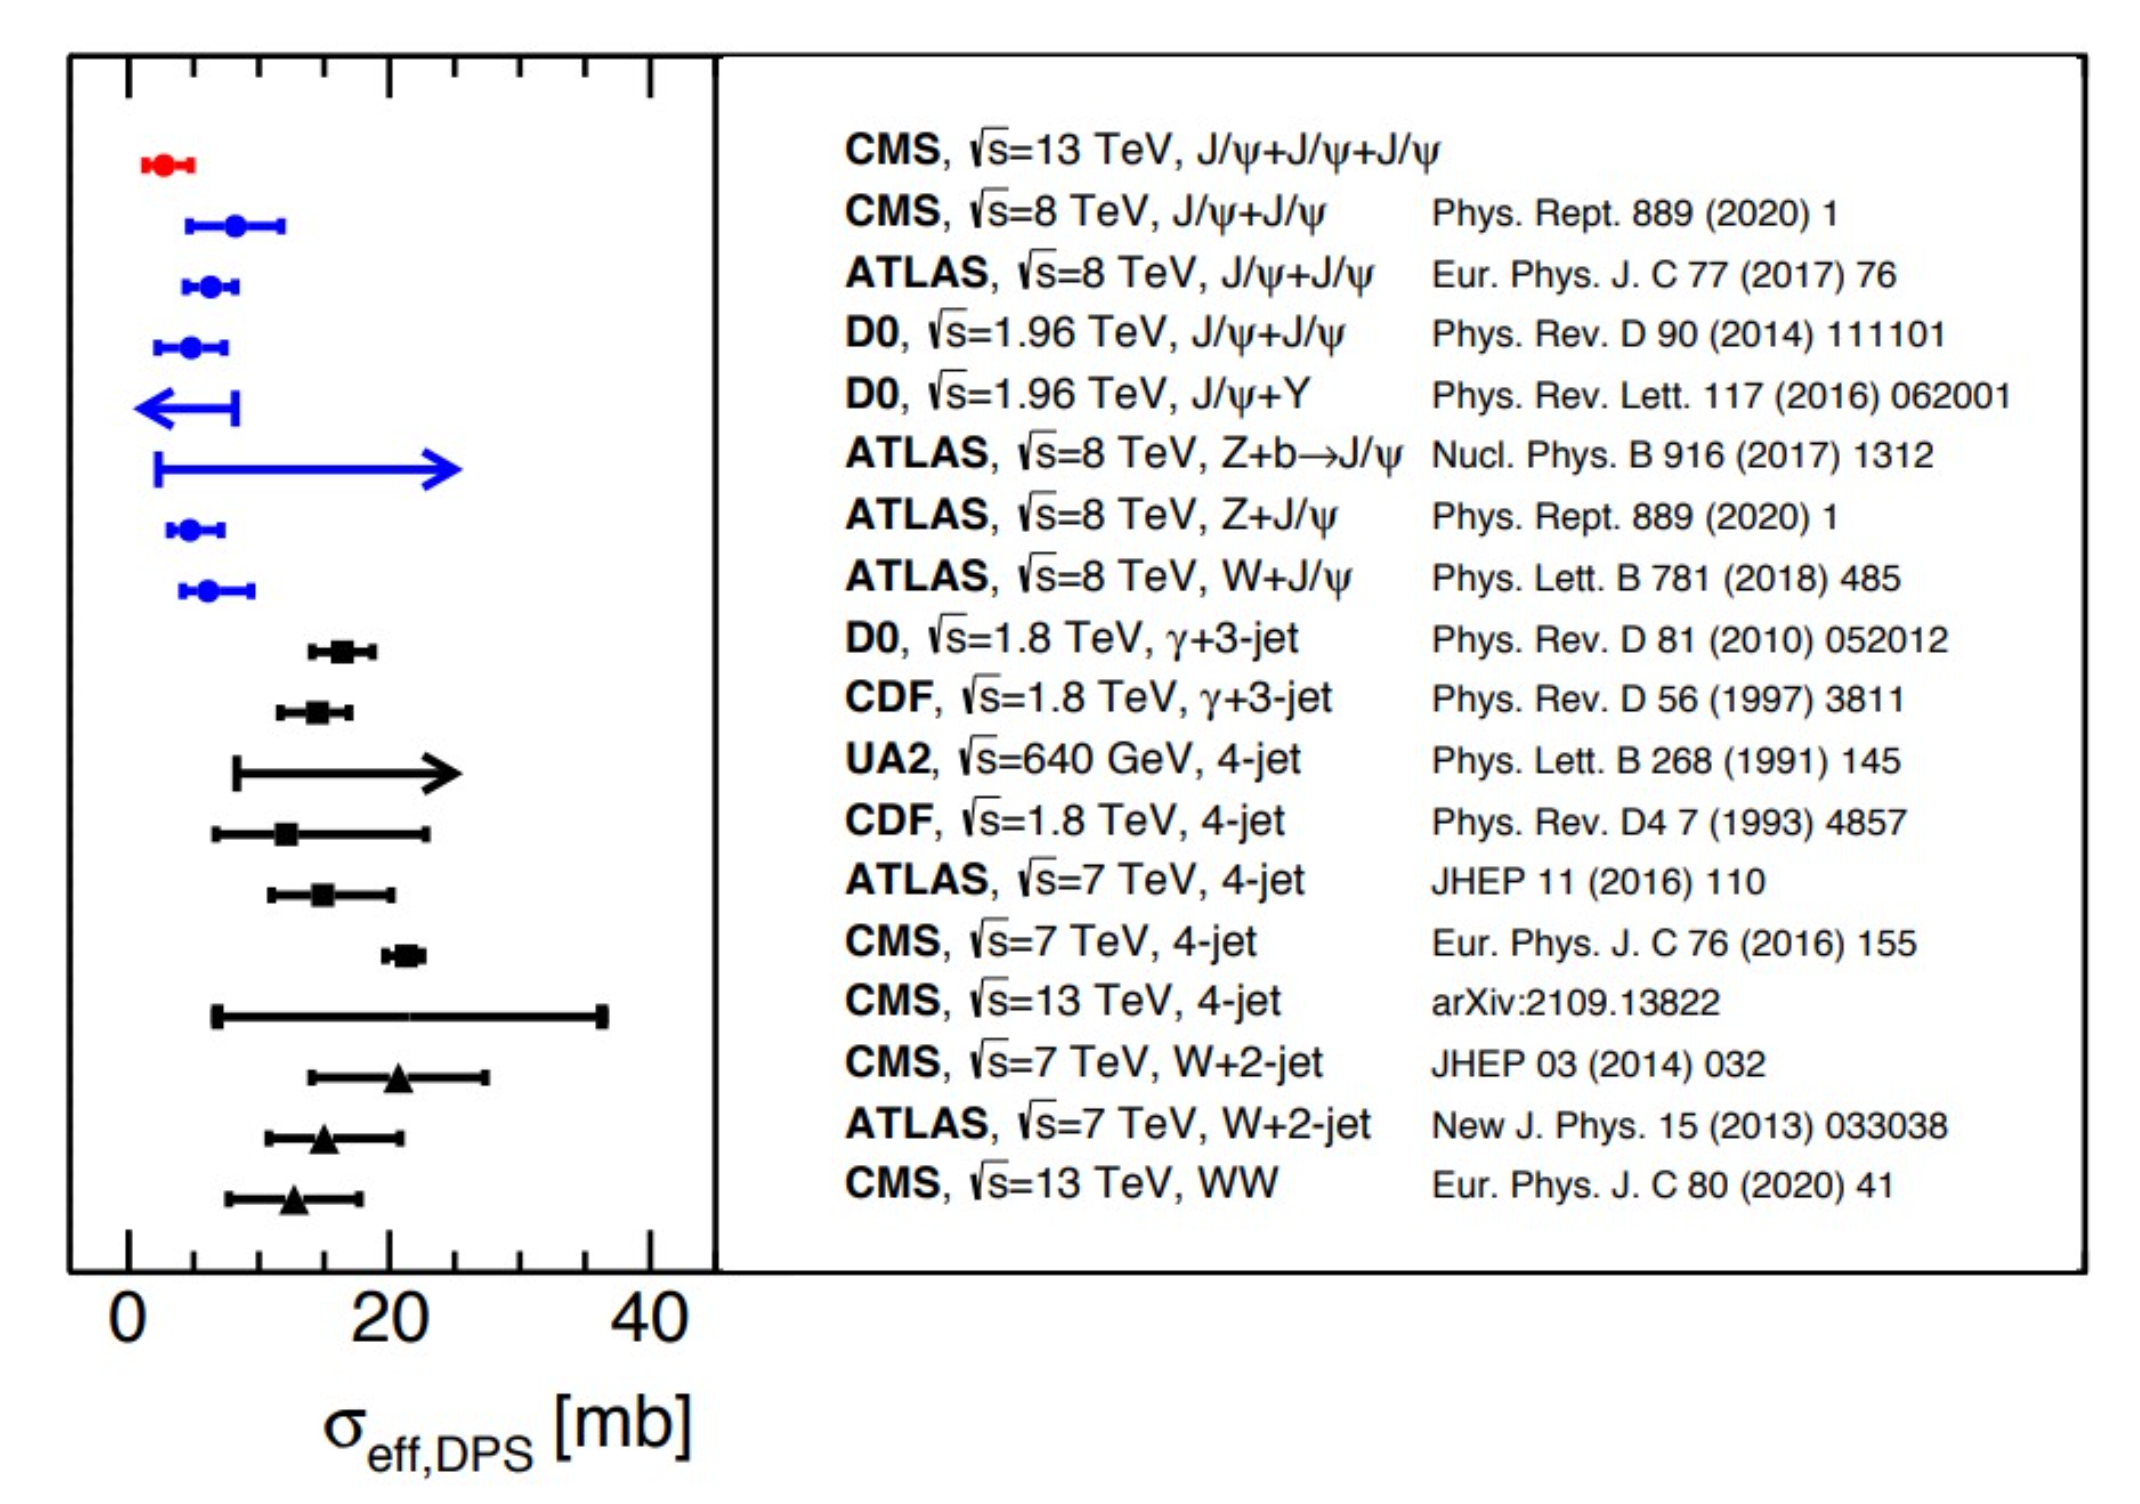
\includegraphics[width=1.0\linewidth]{images/sigma_eff_DPS_summary.png}
    \caption{Summary of current \texorpdfstring{$\effXsecDPS$}{DPS effective cross-section} measurement results in various final states, including results from the triple-$J/\psi$ production process on the top.\cite{CMS_TRI_JPSI}}
    \label{fig:sigma-eff-dps-summary}
\end{figure}

Disagreement in $\effXsecDPS$ obtained in different methods has been interpreted as from the difference in the dominant parton species probed through such processes \cite{MPI_LHC}, yet in some cases it could also be explained by inadequate SPS component subtraction.
Proposals such as measuring associated production of low-$p_T$ $Z$ boson with two jets, or studying the same-sign W boson pair productions have been put forward to improve the purity of DPS event extraction.\cite{andersenExploringHighPurityMultiparton2024}\cite{kuleszaLikesignBosonProduction2000}
Beyond the DPS processes, triple parton scattering (TPS) processes offer another avenue for exploring the proton structure.

\section{Triple Parton Scattering}

TPS processes in high-energy proton-proton collisions have drawn much attention both in theory and experiments.
In a theoretical work by D. d'Enterria and A. M. Snigirev \cite{DdE_TPS}, it was derived from numerous transverse parton density distributions that, for a DPS processes and a TPS process with similar final states, the effective cross-sections $\effXsecDPS, \effXsecTPS$ satisfy the following relationship:

\begin{equation}
    \label{eqn:dps_tps_eff_xsec}
    \effXsecTPS = \kappa \effXsecDPS \quad (\kappa = 0.82 \pm  0.11)
\end{equation}

A more specific study on TPS processes was conducted by H.-S.
Shao and Y.-J. Zhang in 2019\cite{YJZ_TRI_JPSI}, in which they demonstrated the feasibility of using existing data to observe triple-$J/\psi$ hadroproduction and, using this process, to probe into TPS processes.
A further work by Y.-J. Zhang demonstrated the feasibility of observing simultaneous production of $J/\psi$, $\Upsilon$ and a $\phi$ meson with $p_T > 2\GeVc$ in high-energy proton-proton collisions\cite{YJZ_MPS_REPORT}.

The triple-$J/\psi$ production in proton-proton collision was soon observed at the CMS experiment, with a DPS effective cross-section of $\effXsecDPS = 2.7^{+1.4}_{-1.0}(\text{exp})^{+1.5}_{-1.0}(\text{theo}) ~\text{mb}$, compatible with previous $\effXsecDPS$ results from di-quarkonia processes.\cite{CMS_TRI_JPSI}

\section{Conclusions}

$n$-parton scattering processes provide a unique window into the internal structure of the proton, allowing us to probe correlations between partons that are not accessible through direct theoretical calculations. While double parton scattering (DPS) has been extensively studied, discrepancies in the extracted effective cross-section $\effXsecDPS$ across different final states suggest a need for more comprehensive measurements and refined theoretical frameworks.

Triple parton scattering (TPS) represents the next frontier in this field, offering a complementary approach to understanding the proton structure. Extending TPS studies, particularly through final states including $J/\psi$, $\Upsilon$, or $\phi$ mesons, will provide critical insights into the underlying parton dynamics. Data taken from LHC Run 3, with unprecedented energy of $\sqrt{s} = 13.6\TeV$ and integrated luminosity, will offer new opportunities to unfold the complexities of parton dynamics within the proton.

\bibliographystyle{unsrt}
\bibliography{mainTemplatePDF.bib}
\end{document}
